\documentclass[11pt,a4paper]{article}

\usepackage{titling}
\usepackage[hidelinks]{hyperref}
\usepackage{graphicx}
\usepackage{grffile}
\usepackage{float}
\usepackage{geometry}

\newcommand{\subtitle}[1]{
	\posttitle{
		\par\end{center}
	\begin{center}\large#1\end{center}
	\vskip0.5em}
}

\begin{document}
	
\title{Hyper Perform\\ Architectural Requirements Specification}
\subtitle{ Organisation: \url{https://github.com/Hyperperform}}
\begin{figure}
	\centering
	
\includegraphics[height=200px]{../Images/CodusMaximus_logo.jpg}
\end{figure}


\author{
	\textbf{Developers:} \\
	Claudio Da Silva	\emph{14205892}	\\
	Rohan Chhipa		\emph{14188377}	\\
	Avinash Singh		\emph{14043778}	\\
	Jason Gordon		\emph{14405025}	\\\\
}

\date{\textbf{Updated \today}}

\maketitle
\thispagestyle{empty}
\pagebreak

\tableofcontents
\pagebreak

\section{Software Architecture Scope}
\begin{figure}[H]
	\begin{center}
		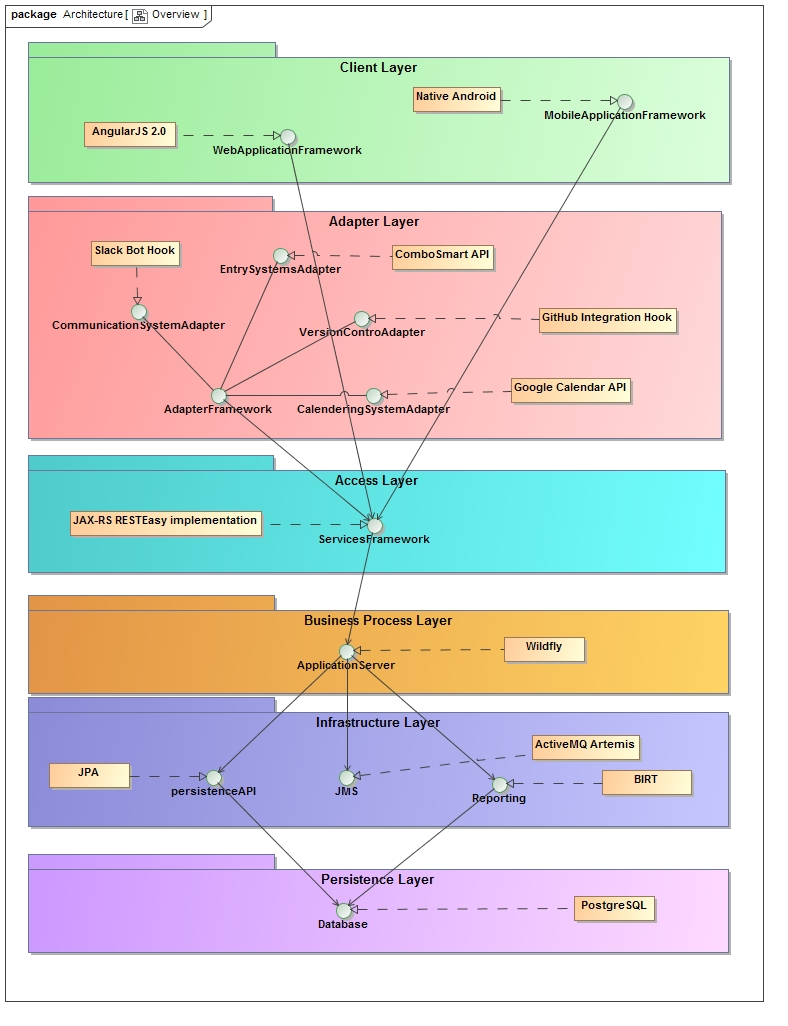
\includegraphics[scale=0.4]{../Images/Architecture_Overview.jpg}
		\caption{A high level break-down of the architecture to be used}
	\end{center}
\end{figure}

\pagebreak

An explanation of some of the adapters follow:
\begin{itemize}
	\item The EntrySystemsAdapter, provides an interface on to which various entry systems such as card readers, biometric scanners and the like can map.
	\item The VersionControlAdapter, provides an interface on to which various version control systems such as GitHub, BitBucket and GitLab can map.
	\item The CalenderingSystemAdaoter, provides an interface for various calendering systems such as Google Calender, or Outlook calender can map on to.
	\item The CommuncationsSystemAdapter, provides an interface on to which various communication systems such as Slacks may map on to.\\\\
\end{itemize}

Extended release adapters will include:
\begin{itemize}
	\item The BugSystemAdapter, which should provide an interface for bug tracking systems such as Waffle.io or Trello to map on to.
	\item The WearablesAdapter, which should provide an interface for wearable devices such as Fitbits and Samsung Gears can map on to.\\\\ 
\end{itemize}

Further information will be provided under integrations.

\pagebreak

\section{Overall Software Architecture}

\subsection{Quality Requirements}
The following section will focus on the quality requirements of the overall system at it's highest level of granularity, and all the requirements defined are defined for all components of the system.

\subsubsection{Flexibility}
The most important element of the system's flexibility is the ability to easily add extra integrations, the main focus of the software is required to source data from various integrations that change with the current market trends and business environment. Thus the need for additional integrations and replacement of default integrations will arise, allowing for a system fully embracing the concept of Internet of Things.\\
The system should be decoupled in the way that it is not limited to specific architectures, thus it should not be locked down to a specific provider for either the application server, the database, or the reporting.

\subsubsection{Maintainability}
An important part of this system is the maintainability of the system, to the extent that the system should be easy for future contributors to change, maintain and further develop.
\begin{itemize}
	\item Future developers should be able to easily understand the system, and modify it as needed.
	\item The technologies chosen for the system can be reasonably expected to be available for a long time as well as remain open source and available.
	\item The system should be able to be maintained without the need to go down for said maintenance, following the always-up methodology.
\end{itemize}

\subsubsection{Integrability}
The system should allow for easy future integration requirements by providing access to it's services using public standards. All external systems should have a preprocessor interface on which to communicate and map on to.

\subsubsection{Scalability}
The system should theoretically be usable in large industries of thousands of employees. Thus the system should be able to handle the load and grow as needed. To accomplish this we make use of the message bus architecture.

\subsubsection{Reliability}
The system should be reliable in the fact that many events will be constantly captured, and in the event a system is not able to currently accept an event, that event must not disappear, but must instead remain on a message queue until the system is able to handle it.

\subsubsection{Security}
\begin{itemize}
	\item Proper authentication should be preformed in order to gain access to confidential user information from the database. 
	\item The messages and the message queue as a whole should be protected from attack from outside systems.
	\item Outside components should only gain access through the message channel, and only when authorised to do so.
\end{itemize}

\subsubsection{Auditability}
Logging should occur for:
\begin{itemize}
	\item Events captured into the queue.
	\item Access to the users personal information.
	\item Generation of reports.
\end{itemize}
Logs should contain at least for all different logs:
\begin{itemize}
	\item An id pertaining to user performing the task.
	\item A description of the activity happening.
	\item The time at which this activity happened.
\end{itemize}

\subsubsection{Usability}
The system should be intuitive and easy to use, the system should not be difficult for a user to learn or interact with. Some things that should be emphasised are:
\begin{itemize}
	\item Useful and helpful error messages, as well as client side validation as far as possible.
	\item Ease of use motions such as swipe where possible.
	\item Labels and hints where possible to guide users.
\end{itemize}

\subsubsection{Testability}
The system must be testable through Continuous Integration using:  
\begin{itemize}
	\item Automated isolated tests using mocks
	\item Automated integration tests using the actual realizations 
\end{itemize}
Tests should ensure that all pre and post-conditions are properly met.

\subsubsection{Deployability}
\begin{itemize}
	\item The system must be built using only the build tool and scripts.
	\item The system should be deployable on cross platform environments.
	\item The system should be deployable in environments with different databases and message brokers.
	\item The system is eventually to be Dockerised for easy distribution. 
\end{itemize}

\pagebreak

\subsection{Architectural Constraints}
The following constraints are non-negotiable and must be met for the system to properly meet client requirements:
\begin{itemize}
	\item The system should be platform independent, allowing for docker to handle the environment setup.
	\item All software used in the creation of this project, including frameworks, libraries and application servers should be strictly open source, as well as preferably well supported and long term.
	\item The web interface should run correctly on all Webkit enabled browsers, and the mobile component should support at least the past three versions of the Android OS.
\end{itemize}

\pagebreak

\subsection{Integration and Access Channels}
In terms of access channels, the project as it stands focuses on two main forms of access:
\begin{itemize}
	\item The web-client component, which will make use of REST calls in order to interact with the back end server. The web client is written in AngularJS 2.0, and interacts with the JavaEE server using the Jersey implementation of REST wrapping.
	\item The Android-client. The Android client similarly makes use of Gradle to retrieve the Maven artefacts needed, and then connects to the JavaEE back end via the same REST wrapping protocols as the web container.\\\\
\end{itemize}
With regards to integration, the system has the following adapters on which to map external integrations on to :
\begin{itemize}
	\item The EntrySystemsAdapter, provides an interface on to which various entry systems such as card readers, biometric scanners and the like can map.
	\item The VersionControlAdapter, provides an interface on to which various version control systems such as GitHub, BitBucket and GitLab can map.
	\item The CalenderingSystemAdaoter, provides an interface for various calendering systems such as Google Calender, or Outlook calender can map on to.
	\item The CommuncationsSystemAdapter, provides an interface on to which various communication systems such as Slacks may map on to.
	
	\item Similarly the event that are retrieved will come through the REST wrapping designed specifically for the events. Each system will
	have its own REST URL to which it will send events. \\\\
\end{itemize}

Thus since the events come through the REST URL's we don't have to continuously poll these systems. Instead the seperate systems send the events when ready. Once the events are received they are processed and placed on a messaging queue.

\pagebreak

\section{Architectural Design}
\subsection{Architectural Tactics}
At the system level of granularity, that being the highest level of granularity, we do not specify any architectural tactics in order to concretely address the quality requirements for the system.
\subsection{Architectural Patterns}
Some of the patterns used at the system level include:
\begin{itemize}
	\item The layered pattern, which limits access of component within one layer to components which are either in the same or the next lower level layer. A great strength it has is that a can be relatively easily replaced. In particular, one can add further access channels without changing any lower layers (A critical component of this system) within the software system and changing the persistence provider would only require changing the persistence API.
	\item The Message Bus pattern, an enterprise integration pattern which allows for safe and efficient handling of events via messages, using a response and request queue, one can ensure that events and messages never get lost even if part of a system fails, thus allowing a greater fail safe in the system.
\end{itemize}
\subsection{Reference Architectures}
The key architecture at the system level is the Enterprise Service Bus. In order to properly network all devices in a proper IOT(Internet of Things) manner, one would implement a message queue system. We chose ActiveMQ Artemis as our realization of this pattern, as it integrates quite nicely into JavaEE, especially the WildFly server we plan to run, and has decent support, as well as many features we can make use of.

\pagebreak

\section{Mobile Access}
It was chosen to use Android Application Framework as the go to mobile access for this project, the reason being that:
\begin{itemize}
	\item Android is the most popularly used mobile OS in the market today
	\item Android has less strings attached, and therefore makes it easier to design, not requiring specific environments in which to build, and has a higher cost for application maintenance.
	\item Many open-source frameworks are available from the community, and many plug-ins and intents are available to make coding easier.
	\item Android provides easier IOT(Internet of Things) structure, via their Samsung Hub, allowing for better integration with other devices later on.\\
\end{itemize}
The build tool to be used for Android will be Gradle, integrated with a Maven repository via Maven dependencies in the Gradle build file.

\pagebreak
	
\section{Technologies}
\subsection{Back end}
\begin{itemize}
	\item WildFly as the JavaEE container and server.
	\item JUnit as a unit testing framework along with Spring.
	\item AspectJ as an Aspect Oriented Programming approach.
	\item RESTEasy implementation of JAX-RS for REST wrapping.
	\item ActiveMQ Artemis as the message broker for the system.
	\item Esper for complex event processing (CEP).
	\item Scala for functional programming on mathematical algorithms.
\end{itemize}
\subsection{Front end}
\begin{itemize}
	\item HTML5, CSS/SCSS and SASS, Bootstrap and JQuery.
	\item AngularJS 2.0 will be used to access the REST services.
	\item BIRT as a front end reporting tool, mixed with ChartJS to create appealing reports.
	\item Android Application Framework, for developing native Android applications.
\end{itemize}
\subsection{Persistence}
\begin{itemize}
	\item PostgreSQL for the database.
	\item JPA as an Object Relational Mapper.
\end{itemize}
\subsection{Deployment tools}
\begin{itemize}
	\item Docker as a shipping container.
	\item TravisCI as a Continuous Integration tool.
\end{itemize}

\end{document}